\documentclass[11pt]{article}
\usepackage[margin=1in]{geometry}
\usepackage[T1]{fontenc}
\usepackage{lmodern}
\usepackage{microtype}
\usepackage{amsmath,amssymb,amsthm,mathtools}
\usepackage{booktabs}
\usepackage{enumitem}
\usepackage{algorithm}
\usepackage[noend]{algpseudocode}
\usepackage{tikz}
\usetikzlibrary{automata,positioning,arrows.meta}
\usepackage[colorlinks=true,linkcolor=blue!50!black,citecolor=blue!50!black,urlcolor=blue!50!black]{hyperref}
\usepackage[nameinlink]{cleveref}

\theoremstyle{plain}
\newtheorem{theorem}{Theorem}
\newtheorem{proposition}[theorem]{Proposition}
\newtheorem{lemma}[theorem]{Lemma}
\newtheorem{corollary}[theorem]{Corollary}
\theoremstyle{definition}
\newtheorem{definition}[theorem]{Definition}
\newtheorem{example}[theorem]{Example}
\theoremstyle{remark}
\newtheorem{remark}[theorem]{Remark}

\newcommand{\R}{\mathbb{R}}
\newcommand{\N}{\mathbb{N}}
\newcommand{\E}{\mathbb{E}}
\newcommand{\Prob}{\mathbb{P}}
\newcommand{\doc}{D}
\newcommand{\edit}{\Delta}
\newcommand{\apply}{\oplus}
\newcommand{\letters}{\lambda}
\DeclareMathOperator{\tree}{tree}
\DeclareMathOperator{\key}{key}
\DeclareMathOperator{\dist}{dist}
\DeclarePairedDelimiter{\abs}{\lvert}{\rvert}
\DeclarePairedDelimiter{\norm}{\lVert}{\rVert}

\title{Papilot: Reviewable Agent Edits for \LaTeX{} Manuscripts}
\author{The Papilot Authors}
\date{}

\begin{document}
\maketitle

\begin{abstract}
Papilot is a personal workspace for revising \LaTeX{} papers with an AI agent
and reviewing every resulting change as a PDF difference before it reaches the
manuscript. Each editing task runs in an isolated Git worktree, may be driven
by Codex, Claude or Antigravity, and proceeds in review rounds in which the
author accepts, rejects or comments on individual changes. This note describes
the system as a small formal model. We define review rounds as operators on a
document, give a sufficient condition under which accepted edits commute, and
estimate how often concurrent tasks conflict. We then treat the geometry of the
PDF view: the affine maps between page, viewport and source, why a naive text
layer drifts from the printed words, and how per-word runs bound that error.
Finally we model notes on the PDF, the agent protocol, usage windows and the
Git operations that close the loop. The paper doubles as Papilot's example
manuscript; every equation in it is a place to try a review.
\end{abstract}

\tableofcontents

\section{Introduction}
\label{sec:introduction}

Writing a research paper is a long sequence of small decisions. An agent that
edits \LaTeX{} can propose many of them quickly, but a proposal is only useful
when the author can see what it changes in the typeset paper, decide, and say
why. Papilot organises this loop around three commitments.

\begin{enumerate}[label=(C\arabic*)]
  \item \emph{Isolation.} Every task edits its own Git worktree, never the
    manuscript checkout, so that unreviewed text cannot leak into the paper.
  \item \emph{Typeset review.} Changes are reviewed as differences between two
    compiled PDFs, with the \LaTeX{} source one click away.
  \item \emph{Explicit acceptance.} Only accepted changes are merged into the
    working tree, and every decision can be undone.
  \end{enumerate}

The rest of this note makes these commitments precise. \Cref{sec:model}
models documents, edits and decisions; \cref{sec:conflicts} estimates
conflicts between concurrent tasks; \cref{sec:geometry} covers the PDF view;
\cref{sec:notes} explains how a mark on the page becomes a source location;
\cref{sec:agents} describes the agent protocol and scheduling;
\cref{sec:usage} models usage windows; and \cref{sec:git} closes with the Git
operations available from the workspace.

\section{A model of review rounds}
\label{sec:model}

\subsection{Documents and edits}

We view a manuscript as a finite sequence of source characters over an
alphabet $\Sigma$, $\doc \in \Sigma^{*}$, of length $n = \abs{\doc}$. An
\emph{edit} replaces a half-open range of the source by new text.

\begin{definition}[Edit]
An edit is a triple $e = (a, b, w)$ with $0 \le a \le b \le n$ and
$w \in \Sigma^{*}$. Applying $e$ to $\doc$ gives
\begin{equation}
  \doc \apply e = \doc_{[0,a)} \, w \, \doc_{[b,n)},
  \label{eq:apply}
\end{equation}
whose length is $n - (b - a) + \abs{w}$.
\end{definition}

A task proposes a \emph{revision} $\edit = \{e_1, \dots, e_m\}$, a finite set
of edits against the same base document. Papilot groups nearby edits into
\emph{changes}, the units the author decides on.

\begin{definition}[Compatibility]
Two edits $e = (a, b, w)$ and $e' = (a', b', w')$ are \emph{compatible},
written $e \perp e'$, when their ranges are disjoint and not adjacent:
\begin{equation}
  e \perp e' \iff b < a' \ \text{or}\ b' < a .
  \label{eq:compatible}
\end{equation}
A revision is compatible when its edits are pairwise compatible.
\end{definition}

For a compatible revision we apply edits from right to left, so that earlier
offsets remain valid:
\begin{equation}
  \doc \apply \edit
  = \bigl(\cdots\bigl((\doc \apply e_{\sigma(1)}) \apply e_{\sigma(2)}\bigr)
    \cdots\bigr) \apply e_{\sigma(m)},
  \qquad a_{\sigma(1)} > a_{\sigma(2)} > \dots > a_{\sigma(m)} .
  \label{eq:apply-revision}
\end{equation}

\begin{proposition}[Compatible edits commute]
\label{prop:commute}
If $e \perp e'$, then applying them right to left in either listing gives the
same document, and the result does not depend on how the remaining edits of a
compatible revision are ordered.
\end{proposition}

\begin{proof}
Assume without loss of generality $b < a'$. Applying $e'$ first changes only
positions at or after $a'$, so the range $[a, b)$ and every offset before it are
unchanged, and applying $e$ afterwards gives
$\doc_{[0,a)}\, w\, \doc_{[b,a')}\, w'\, \doc_{[b',n)}$. Applying $e$ first
shifts every later offset by $\delta = \abs{w} - (b-a)$; rewriting $e'$ as
$(a'+\delta, b'+\delta, w')$ yields the same string. Induction on the number of
edits, ordering them by start offset, gives the general statement.
\end{proof}

\subsection{Decisions and rounds}

Let $U$ be the set of changes in a round. A \emph{decision state} is a map
\begin{equation}
  \theta : U \to \{\textsf{pending}, \textsf{accepted}, \textsf{rejected},
  \textsf{commented}\},
\end{equation}
and the accepted part of a revision is
$\edit^{\theta} = \{ e \in \edit : \theta(u(e)) = \textsf{accepted} \}$.
The manuscript after round $t$ is
\begin{equation}
  \doc_{t+1} =
  \begin{cases}
    \doc_t \apply \edit_t^{\theta_t}, & \text{if } \edit_t^{\theta_t}
      \text{ applies cleanly to } \doc_t,\\[2pt]
    \doc_t, & \text{otherwise, and the task is asked for a new proposal.}
  \end{cases}
  \label{eq:round}
\end{equation}
Rejected and commented changes return to the agent as feedback bound to their
round, file and lines; the agent must not reintroduce a rejected edit unless it
is explicitly asked to.

\begin{remark}
Undo restores the previous decision state $\theta_{t}$ and the corresponding
working tree. Decisions are idempotent: replaying an action with the same
identifier has no further effect, which is what makes an uncertain network
write safe to retry.
\end{remark}

\subsection{How many rounds?}

Suppose that each change is accepted in a round independently with probability
$p \in (0,1]$, and otherwise revised and proposed again. The number of rounds
$R$ until a single change is accepted is geometric,
$\Prob(R = r) = (1-p)^{r-1} p$, so $\E[R] = 1/p$. For $m$ independent changes
the task ends when the last one is accepted, after
$R_{\max} = \max_i R_i$ rounds, and inclusion--exclusion gives
\begin{equation}
  \E[R_{\max}]
  = \sum_{r \ge 0} \Prob(R_{\max} > r)
  = \sum_{r \ge 0} \Bigl(1 - \bigl(1 - (1-p)^{r}\bigr)^{m}\Bigr)
  = \sum_{k=1}^{m} (-1)^{k+1} \binom{m}{k} \frac{1}{1 - (1-p)^{k}} .
  \label{eq:rounds}
\end{equation}
For small $p$ this behaves like $\frac{1}{p} H_m$, where
$H_m = \sum_{k=1}^{m} 1/k \approx \ln m + \gamma$ is the $m$-th harmonic
number: doubling the number of changes adds only about $(\ln 2)/p$ rounds.

\begin{example}
With $p = 0.8$ and $m = 5$, \cref{eq:rounds} gives
$\E[R_{\max}] \approx 1.91$: most tasks finish in one or two rounds.
\end{example}

\section{Concurrent tasks and conflicts}
\label{sec:conflicts}

Papilot runs up to $c = 2$ tasks at once, each against the manuscript as it was
when the task started. Accepted text from one task can therefore overlap a
later proposal from another.

\begin{proposition}[Conflict probability]
\label{prop:conflict}
Let two tasks propose $k_1$ and $k_2$ edits, each covering $\ell$ characters at
positions chosen independently and uniformly in a document of length
$n \gg \ell$. The probability that some pair of edits from different tasks is
incompatible is
\begin{equation}
  \Prob(\text{conflict})
  = 1 - \Bigl(1 - \frac{2\ell + 1}{n}\Bigr)^{k_1 k_2}
  \approx 1 - \exp\Bigl(-\frac{(2\ell+1)\, k_1 k_2}{n}\Bigr).
  \label{eq:conflict}
\end{equation}
\end{proposition}

\begin{proof}
Two edits of length $\ell$ starting at $s$ and $s'$ violate
\cref{eq:compatible} exactly when $\abs{s - s'} \le \ell$, an event of
probability $(2\ell+1)/n$ up to boundary effects of order $\ell/n$. There are
$k_1 k_2$ cross pairs; treating them as independent gives the product, and
$\log(1-x) = -x + O(x^2)$ gives the approximation.
\end{proof}

For a $40$-page paper with $n \approx 1.2 \times 10^{5}$ characters, two tasks
of $k_1 = k_2 = 10$ edits of $\ell = 200$ characters conflict with probability
about $1 - e^{-0.33} \approx 0.28$. Papilot surfaces such conflicts from Git
rather than resolving them, in keeping with~\eqref{eq:round}.

\section{Building the PDF}
\label{sec:build}

The PDF view shows the manuscript exactly as it is on disk, including accepted
but uncommitted changes. Let $W$ be the working tree and $H$ the tree of
\texttt{HEAD}. A temporary index $I$ records the working tree without touching
the real index:
\begin{equation}
  I \leftarrow \operatorname{read-tree}(H), \qquad
  I \leftarrow I \cup \operatorname{add}(W), \qquad
  T = \operatorname{write-tree}(I) .
\end{equation}
The build is cached under the key
\begin{equation}
  \key(W) = h\bigl(T \,\|\, \text{build settings}\bigr),
\end{equation}
where $h$ is a cryptographic hash. Because $T$ depends only on content, two
working trees with the same files share a build: undoing a decision returns to
a tree that has already been built, and the PDF reappears without compiling.

\section{Geometry of the PDF view}
\label{sec:geometry}

\subsection{From page to screen}

A PDF page lives in user space, in points ($1\,\mathrm{pt} = 1/72$\,in), with
the origin at the bottom left of its view box $[x_0, y_0, x_1, y_1]$. The
viewer draws it at scale $s$ (device pixels per point) with the origin at the
top left, so for an unrotated page the map to screen coordinates is the affine
transform
\begin{equation}
  \begin{pmatrix} u \\ v \\ 1 \end{pmatrix}
  =
  \begin{pmatrix}
    s & 0 & -s x_0 \\
    0 & -s & s y_1 \\
    0 & 0 & 1
  \end{pmatrix}
  \begin{pmatrix} x \\ y \\ 1 \end{pmatrix} .
  \label{eq:viewport}
\end{equation}
A rotation by $\phi \in \{0, \tfrac{\pi}{2}, \pi, \tfrac{3\pi}{2}\}$ composes
this with $\begin{psmallmatrix} \cos\phi & -\sin\phi \\ \sin\phi & \cos\phi
\end{psmallmatrix}$ about the page centre. Notes are stored in normalised
coordinates $r = (\xi_0, \eta_0, \xi_1, \eta_1) \in [0,1]^4$ relative to the
page box, so that they survive any zoom:
\begin{equation}
  \xi = \frac{x - x_0}{x_1 - x_0}, \qquad
  \eta = \frac{y_1 - y}{y_1 - y_0} .
\end{equation}

\subsection{Why a naive text layer drifts}

To make text selectable, a viewer overlays invisible text on the rendered page.
A common construction places one run per line in a stand-in font and stretches
it horizontally so that the run's ends meet the line's ends. Let a line consist
of glyphs with true advances $a_1, \dots, a_N$ and stand-in advances
$b_1, \dots, b_N$. The stretch factor is
\begin{equation}
  \sigma = \frac{\sum_{i=1}^{N} a_i}{\sum_{i=1}^{N} b_i},
\end{equation}
and the selectable position of glyph $k$ is off by
\begin{equation}
  \varepsilon_k = \sum_{i<k} \bigl(\sigma b_i - a_i\bigr), \qquad
  \varepsilon_1 = \varepsilon_{N+1} = 0 .
  \label{eq:drift}
\end{equation}

\begin{proposition}[Mid-line drift]
\label{prop:drift}
If the per-glyph discrepancies $\delta_i = \sigma b_i - a_i$ behave like
independent zero-mean variables of variance $\tau^2$, conditioned on
$\sum_i \delta_i = 0$, then $(\varepsilon_k)$ is a discrete Brownian bridge and
\begin{equation}
  \E\bigl[\varepsilon_k^2\bigr] = \tau^2\, \frac{(k-1)(N-k+1)}{N},
  \qquad
  \max_k \E\bigl[\varepsilon_k^2\bigr] \approx \frac{\tau^2 N}{4} .
  \label{eq:bridge}
\end{equation}
\end{proposition}

\begin{proof}
Without the constraint, $\varepsilon_k$ is a random walk with variance
$(k-1)\tau^2$. Conditioning a Gaussian walk on returning to zero at step
$N+1$ gives $\operatorname{Var}(\varepsilon_k) = \tau^2 (k-1)(N-k+1)/N$, which
is maximal in the middle of the line.
\end{proof}

Justified \LaTeX{} lines add a second source of error: the stretchable glue
between words. If the natural interword space is $g$ and the line is set with
stretch ratio $\rho$, every space is $g(1+\rho)$ wide in print but $b_{\text{space}}$
in the stand-in font, which adds a deterministic bias of
\begin{equation}
  \beta_k = \bigl(g(1+\rho) - \sigma b_{\text{space}}\bigr) \cdot
  \#\{\text{spaces before } k\} .
\end{equation}
Together, \cref{eq:bridge} and $\beta_k$ explain drifts of several characters
in the middle of a line, enough for a drag to select a neighbouring word.

\subsection{Per-word runs}

Papilot instead reads every word's printed place from the PDF (its left edge
$\lambda_j$, baseline $y_j$, size $f_j$ and width $w_j$) and places one run per
word, stretched to end where the next word begins. The error is then confined
to a single word $j$ of $N_j$ glyphs:
\begin{equation}
  \abs{\varepsilon_k} \le \max_{i \in j} \abs{\delta_i} \cdot N_j,
  \qquad
  \E\bigl[\varepsilon_k^2\bigr] \le \frac{\tau^2 N_j}{4}
  \ll \frac{\tau^2 N}{4},
\end{equation}
and every word starts exactly where it is printed. For a line of $N = 80$
glyphs and words of $N_j \approx 6$, the typical error falls by a factor of
about $\sqrt{N / N_j} \approx 3.7$, and the bias $\beta_k$ disappears.

\section{Notes on the PDF}
\label{sec:notes}

\subsection{From a mark to source lines}

A note is a set of rectangles $\{r_1, \dots, r_q\}$ on page $P$ together with a
comment. For every line the selection touches, Papilot asks SyncTeX for the
source position of the first and last marked character~\cite{laurens2008}:
\begin{equation}
  \mathcal{S}(P, x, y) = (\text{file}, \text{line}),
  \qquad
  L = \{\, \mathcal{S}(P, c) : c \in C_{\text{first}} \cup C_{\text{last}} \,\},
  \qquad
  [\ell_{-}, \ell_{+}] = [\min L, \max L].
\end{equation}

SyncTeX records boxes and glue rather than characters. The space before a word
that begins a printed line comes from the line break of the \emph{previous}
source line, so such a word is credited to that line. Papilot therefore
\emph{settles} each end of the selection by matching its printed context
against the source near SyncTeX's answer.

Let $\letters(\cdot)$ map text to its lowercase letters and digits, after
Unicode compatibility normalisation, with \TeX{} control sequences and comments
removed from the source. For a source window $[\ell_{-} - 4, \ell_{+} + 4]$ we
form the string $S = \letters(\text{lines})$ and remember for each position the
line it came from, $\pi : \{1, \dots, \abs{S}\} \to \N$. The distance of a
line from SyncTeX's range is
\begin{equation}
  \dist(\ell) = \max\bigl(0,\ \ell_{-} - \ell,\ \ell - \ell_{+}\bigr).
\end{equation}

\begin{algorithm}[t]
\caption{Settling one end of a selection}
\label{alg:settle}
\begin{algorithmic}[1]
\Require printed line $p$, index $\alpha$ of the marked letter in $\letters(p)$, source string $S$ with line map $\pi$
\For{$\rho \in (\infty, 24, 10)$} \Comment{whole line first, then shorter context}
  \State $q \gets \letters(p)_{[\alpha - \rho,\ \alpha + \rho]}$
  \State $O \gets \{ o : S_{[o,\, o + \abs{q})} = q \}$
  \If{$O \neq \emptyset$}
    \State $o^{\star} \gets \arg\min_{o \in O} \dist\bigl(\pi(o + \alpha - \max(0, \alpha - \rho))\bigr)$
    \State \Return $\pi\bigl(o^{\star} + \alpha - \max(0, \alpha - \rho)\bigr)$
  \EndIf
\EndFor
\State \Return SyncTeX's line \Comment{formulas and other unmatched text}
\end{algorithmic}
\end{algorithm}

\Cref{alg:settle} runs once for the first and once for the last marked
character. If the settled range is empty or inverted, Papilot keeps SyncTeX's
range. Because the comparison uses letters only, subscripts, macros and
hyphenation do not prevent a match; formulas, whose printed form shares no
letters with their source, fall back to SyncTeX by design.

\subsection{Whole words}

Let a drag select characters $[s, t)$ of the text layer. Papilot widens the
selection to whole words, but only at a boundary that cuts through a word:
\begin{equation}
  s' = \begin{cases}
    \max\{ i \le s : \text{$i = 0$ or $c_{i-1}$ is not a letter} \}, &
      c_s \text{ is a letter},\\
    s, & \text{otherwise},
  \end{cases}
\end{equation}
and symmetrically for $t$. A drag that ends at the start of the next word
therefore keeps exactly the words it covers.

\section{Agents and scheduling}
\label{sec:agents}

\subsection{One protocol for three agents}

Every agent is driven through the same small protocol: a thread is started or
resumed, a turn is started with the author's text, the agent streams items
(messages, commands, file changes, questions), and the turn completes, is
interrupted, or fails. Formally a task moves through the states of
\cref{fig:states}.

\begin{figure}[t]
\centering
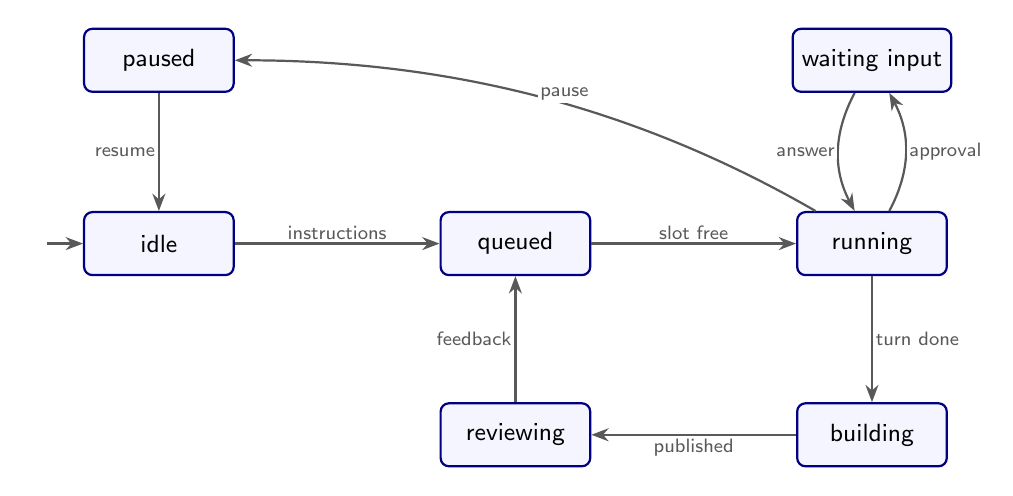
\begin{tikzpicture}[
  >={Stealth[length=2.2mm]}, node distance=2.1cm and 2.6cm,
  every state/.style={draw=blue!50!black, thick, fill=blue!4, rounded corners=3pt,
    rectangle, minimum width=1.9cm, minimum height=0.8cm, font=\small\sffamily},
  every edge/.style={draw, ->, thick, gray!70!black},
  lbl/.style={font=\scriptsize\sffamily, fill=white, inner sep=1pt}]
  \node[state, initial, initial text={}] (idle) {idle};
  \node[state, right=of idle] (queued) {queued};
  \node[state, right=of queued] (running) {running};
  \node[state, below=1.6cm of running] (building) {building};
  \node[state, left=of building] (reviewing) {reviewing};
  \node[state, above=1.5cm of running] (waiting) {waiting input};
  \node[state, above=1.5cm of idle] (paused) {paused};
  \path (idle) edge node[lbl, above] {instructions} (queued)
        (queued) edge node[lbl, above] {slot free} (running)
        (running) edge[bend right=28] node[lbl, right] {approval} (waiting)
        (waiting) edge[bend right=28] node[lbl, left] {answer} (running)
        (running) edge node[lbl, right] {turn done} (building)
        (building) edge node[lbl, below] {published} (reviewing)
        (reviewing) edge node[lbl, left] {feedback} (queued)
        (running) edge[out=150, in=0, looseness=0.9] node[lbl, above, pos=0.45] {pause} (paused)
        (paused) edge node[lbl, left] {resume} (idle);
\end{tikzpicture}
\caption{Task states. A turn that fails or whose outcome is uncertain leaves the
task in a recoverable state with a \emph{Check status} action (not shown).}
\label{fig:states}
\end{figure}

Codex speaks this protocol natively. Claude runs through the Claude Agent SDK,
and Antigravity runs the \texttt{agy} command line once per turn; both are
translated by small adapters. A reasoning effort $\epsilon$ from an ordered
set $\mathcal{E} = \{\textsf{low} < \textsf{medium} < \textsf{high} <
\textsf{xhigh} < \textsf{max}\}$ is chosen per task. If a turn at effort
$\epsilon$ consumes on average $\kappa(\epsilon)$ tokens and succeeds with
probability $q(\epsilon)$, the expected cost of a completed change is
\begin{equation}
  \operatorname{cost}(\epsilon) = \frac{\kappa(\epsilon)}{q(\epsilon)}
  \cdot \operatorname{price}, \qquad
  \epsilon^{\star} = \arg\min_{\epsilon \in \mathcal{E}}
    \operatorname{cost}(\epsilon),
\end{equation}
which explains why a lower effort is not always cheaper: a failed turn must be
paid for again.

\subsection{Queueing}

Tasks arrive at rate $\nu$ and occupy a slot for a mean time $1/\omega$. With
$c$ slots and offered load $A = \nu/\omega < c$, the probability that a new
task waits is given by the Erlang~C formula~\cite{erlang1917}:
\begin{equation}
  C(c, A) =
  \frac{\dfrac{A^{c}}{c!}\,\dfrac{c}{c - A}}
       {\displaystyle\sum_{k=0}^{c-1} \frac{A^{k}}{k!}
        + \frac{A^{c}}{c!}\,\frac{c}{c - A}},
  \qquad
  \E[\text{wait}] = \frac{C(c, A)}{c\,\omega - \nu} .
  \label{eq:erlang}
\end{equation}
For $c = 2$ this simplifies to $C(2, A) = A^2 / (2 + A)$. An author who starts
a task every ten minutes, each taking six minutes, has $A = 0.6$ and waits
with probability about $0.14$.

\section{Usage windows}
\label{sec:usage}

Agent subscriptions meter usage over rolling windows. If $r(\tau)$ is the rate
at which a plan's allowance is consumed, the utilisation of a window of length
$w$ at time $t$ is
\begin{equation}
  u_w(t) = \frac{1}{B_w} \int_{t-w}^{t} r(\tau)\, d\tau \in [0, 1],
\end{equation}
where $B_w$ is the window's budget. Papilot shows $u_w$ for each window the
agent reports, coloured by thresholds
\begin{equation}
  \text{colour}(u) =
  \begin{cases}
    \text{blue}, & u < 0.75,\\
    \text{amber}, & 0.75 \le u < 0.9,\\
    \text{red}, & u \ge 0.9 \ \text{or the limit is reached},
  \end{cases}
\end{equation}
together with the reset time. At a constant rate $\bar r$, the time left before
the limit is $(1 - u_w(t)) B_w / \bar r$; with the weekly window at
$u = 0.83$ and an even pace over the week, about $1.2$ days of work remain.

\section{Closing the loop with Git}
\label{sec:git}

Accepted changes land in the working tree without a commit, so that the author
decides what history to write. Let $\operatorname{HEAD}$ have tree $H$, let
$I$ be the index and $W$ the working tree, and let $P$ be the set of paths the
author ticks. A commit from Papilot produces the tree
\begin{equation}
  T_{c} = H \big|_{\overline{P}} \;\cup\; W \big|_{P},
\end{equation}
that is, exactly the chosen files as they are on disk, while anything staged
for other paths, $I|_{\overline{P}}$, stays staged and out of the commit.
Renames contribute both their old and new paths to $P$.

Pull is a fast-forward only. With local head $L$ and upstream $U$, it succeeds
exactly when
\begin{equation}
  \operatorname{merge-base}(L, U) = L,
\end{equation}
in which case $L \leftarrow U$; otherwise Papilot reports the divergence and
never merges or rebases on the author's behalf. The branch is ahead by
$\abs{\operatorname{rev}(U..L)}$ and behind by $\abs{\operatorname{rev}(L..U)}$
commits, the two numbers shown beside the branch name.

\section{Discussion}
\label{sec:discussion}

Three limitations are worth stating. First, \cref{prop:conflict} assumes
uniformly placed edits; real revisions cluster around the parts of a paper an
author is working on, which raises the conflict rate and argues for fewer,
longer tasks over many short ones. Second, \cref{alg:settle} cannot settle
formulas, since their printed form shares no letters with their source; for
those, SyncTeX's lines are kept and the excerpt shows the whole display.
Third, an agent that cannot ask for permission, such as a headless command
line, must be restricted in advance; Papilot runs such agents so that they edit
only the task's worktree.

\section{Conclusion}

Papilot treats agent editing as a sequence of reviewable rounds. Isolation
makes proposals safe, typeset review makes them legible, and explicit
acceptance keeps the author in charge of the paper. The small amount of
mathematics in this note is there to make those properties checkable, and to
give the reader something worth reviewing.

\appendix

\section{Notation}
\label{app:notation}

\begin{center}
\begin{tabular}{@{}lll@{}}
\toprule
Symbol & Meaning & Where \\
\midrule
$\doc$, $n$ & manuscript source and its length & \cref{sec:model} \\
$e = (a, b, w)$ & edit replacing $[a, b)$ by $w$ & \cref{eq:apply} \\
$e \perp e'$ & compatible edits & \cref{eq:compatible} \\
$\theta$ & decision state of a round & \cref{eq:round} \\
$p$, $R_{\max}$ & acceptance probability, rounds for a task & \cref{eq:rounds} \\
$\ell$, $k_i$ & edit length, edits per task & \cref{eq:conflict} \\
$s$, $[x_0, y_0, x_1, y_1]$ & viewer scale, page view box & \cref{eq:viewport} \\
$\varepsilon_k$, $\sigma$ & text layer drift, stretch factor & \cref{eq:drift} \\
$\mathcal{S}$, $\letters$ & SyncTeX query, letter normalisation & \cref{sec:notes} \\
$c$, $A$ & concurrent slots, offered load & \cref{eq:erlang} \\
$u_w$, $B_w$ & window utilisation and budget & \cref{sec:usage} \\
$H$, $I$, $W$, $P$ & Git trees, index, working tree, chosen paths & \cref{sec:git} \\
\bottomrule
\end{tabular}
\end{center}

\section{Keyboard}
\label{app:keyboard}

\begin{center}
\begin{tabular}{@{}ll@{}}
\toprule
Key & Action \\
\midrule
\texttt{A}, \texttt{R}, \texttt{C} & accept, reject or comment on the current change \\
\texttt{J}, \texttt{K} & next and previous change \\
\texttt{S} & show the \LaTeX{} source of the current change \\
$\text{\texttt{Cmd}} + \text{\texttt{F}}$ & find in the PDF \\
$\text{\texttt{Cmd}} + \text{\texttt{+}}$, $\text{\texttt{Cmd}} + \text{\texttt{-}}$, $\text{\texttt{Cmd}} + \text{\texttt{0}}$ & zoom in, zoom out, fit width \\
\texttt{Enter}, \texttt{Shift+Enter} & send, new line \\
\bottomrule
\end{tabular}
\end{center}

\begin{thebibliography}{9}
\bibitem{laurens2008}
J.~Laurens.
\newblock Direct and reverse synchronization with Sync\TeX.
\newblock \emph{TUGboat}, 29(3):365--371, 2008.

\bibitem{erlang1917}
A.~K. Erlang.
\newblock Solution of some problems in the theory of probabilities of
  significance in automatic telephone exchanges.
\newblock \emph{Elektroteknikeren}, 13:5--13, 1917.

\bibitem{chacon2014}
S.~Chacon and B.~Straub.
\newblock \emph{Pro Git}.
\newblock Apress, second edition, 2014.

\bibitem{knuth1984}
D.~E. Knuth.
\newblock \emph{The \TeX book}.
\newblock Addison-Wesley, 1984.
\end{thebibliography}

\end{document}
